\documentclass[12pt, twoside]{article}
\usepackage[letterpaper, margin=1in, headsep=0.2in]{geometry}
\setlength{\headheight}{0.6in}
%\usepackage[english]{babel}
\usepackage[utf8]{inputenc}
\usepackage{microtype}
\usepackage{amsmath}
\usepackage{amssymb}
%\usepackage{amsfonts}
\usepackage{siunitx} %units in math. eg 20\milli\meter
\usepackage{yhmath} % for arcs, overparenth command
\usepackage{tikz} %graphics
\usetikzlibrary{quotes, angles}
\usepackage{graphicx} %consider setting \graphicspath{{images/}}
\usepackage{parskip} %no paragraph indent
\usepackage{enumitem}
\usepackage{multicol}
\usepackage{venndiagram}

\usepackage{fancyhdr}
\pagestyle{fancy}
\fancyhf{}
\renewcommand{\headrulewidth}{0pt} % disable the underline of the header
\raggedbottom
\hfuzz=2mm %suppresses overfull box warnings

\usepackage{hyperref}

\fancyhead[LE]{\thepage}
\fancyhead[RO]{\thepage \\ Name: \hspace{4cm} \,\\}
\fancyhead[LO]{BECA / Dr. Huson / Geometry\\*  Unit 6: Analytic geometry\\* 29 November 2022}

\begin{document}

\subsubsection*{6.5 Homework: Slope \hfill CCSS.HSG.SRT.C.8}
\begin{enumerate}
\item Find the slope of the line $\overleftrightarrow{AB}$, $A(2,1)$, $B(3,4)$. Use the formula and show the substitution step.
\begin{multicols}{2}
  $\displaystyle m = \frac{y_B - y_A}{x_B - x_A}$
    \vspace{2cm}
    \begin{flushright}
    \begin{tikzpicture}[scale=1]
      \draw [help lines] (-1,-1) grid (6,6);
      \draw [thick, ->] (-1.2,0) -- (6.4,0) node [below right] {$x$};
      \draw [thick, ->] (0,-1.2)--(0,6.4) node [left] {$y$};
      \draw [fill] (2,1) circle [radius=0.05] node[above left] {$A(2,1)$};
      \draw [fill] (3,4) circle [radius=0.05] node[above right] {$B(3,4)$};
      \draw [<->, thick] (1,-2)--(4,7);
    \end{tikzpicture}
    \end{flushright}
\end{multicols}

\item Plot the points and find the slope of the line $\overleftrightarrow{RS}$, $R(1,3)$, $S(3,4)$. Use the formula and show the substitution step. As a check, draw the line and count the rise and run.
\begin{multicols}{2}
  $\displaystyle m = \frac{y_S - y_R}{x_S - x_R}$
    \vspace{2cm}
    \begin{flushright}
    \begin{tikzpicture}[scale=1]
      \draw [help lines] (-1,-1) grid (6,6);
      \draw [thick, ->] (-1.2,0) -- (6.4,0) node [below right] {$x$};
      \draw [thick, ->] (0,-1.2)--(0,6.4) node [left] {$y$};
      %\draw [fill] (2,1) circle [radius=0.05] node[above left] {$A(2,1)$};
      %\draw [fill] (3,4) circle [radius=0.05] node[above right] {$B(3,4)$};
      %\draw [<->, thick] (1,-2)--(4,7);
    \end{tikzpicture}
    \end{flushright}
\end{multicols}

\item Find the equation of the given line $\overleftrightarrow{AB}$, $A(0,4)$, $B(4,2)$.
\begin{multicols}{2}
    \begin{enumerate}[itemsep=1cm]
      \item Find the slope, $m$, showing the substitution step in the slope formula: \\[0.5cm]
      $\displaystyle m = \frac{y_B - y_A}{x_B - x_A}$\\[0.5cm]
      \item Write down the $y$-intercept.
      \item Write the equation of the line in the slope-intercept form\\[0.25cm]
      $y=mx+b$
      \end{enumerate}
    \begin{flushright}
    \begin{tikzpicture}[scale=0.8]
      \draw [help lines] (-1,-1) grid (6,6);
      \draw [thick, ->] (-1.2,0) -- (6.4,0) node [below right] {$x$};
      \draw [thick, ->] (0,-1.2)--(0,6.4) node [left] {$y$};
      \draw [fill] (0,4) circle [radius=0.05] node[above right] {$A(0,4)$};
      \draw [fill] (4,2) circle [radius=0.05] node[above right] {$B(4,2)$};
      \draw [<->, thick] (-1,4.5)--(5.5,1.25);
    \end{tikzpicture}
    \end{flushright}
  \end{multicols}

\item Complete each statement about linear equations.
\begin{enumerate}[itemsep=0.5cm]
  \item What is the slope of a horizontal line?
  \item What is the $y$-intercept of the line $y = 2x + 3$?
  \item What is the slope of the line $y = x - 5$?
  \item Which has an undefined slope, a vertical or horizontal line?
  \item What is the $y$-intercept of the line $y = -2x$?
\end{enumerate}

\item Two parallel lines are shown in the graph, $p$ and $q$.
\begin{multicols}{2}
    \begin{enumerate}[itemsep=1cm]
      \item Find the slope, $m$, by counting squares across and up on the line. \\[0.5cm]
      $\displaystyle m = \frac{rise}{run}$\\[0.5cm]
      \item True or false: parallel lines have equal slopes.
      \item Write the slope of a line perpendicular to $p$ (the negative reciprocal).\\[0.25cm]
      $m_{\perp}=$
      \end{enumerate}
    \begin{flushright}
    \begin{tikzpicture}[scale=0.9]
      \draw [help lines] (-1,-1) grid (6,6);
      \draw [thick, ->] (-1.2,0) -- (6.4,0) node [below right] {$x$};
      \draw [thick, ->] (0,-1.2)--(0,6.4) node [left] {$y$};
      %\draw [fill] (0,4) circle [radius=0.05] node[above right] {$A(0,4)$};
      %\draw [fill] (4,2) circle [radius=0.05] node[above right] {$B(4,2)$};
      \draw [<->, thick] (-0.5,2.75)--(6.5,6.25) node [below]{$p$};
      \draw [<->, thick] (-0.5,0.75)--(6.5,4.25) node [below]{$q$};
    \end{tikzpicture}
    \end{flushright}
\end{multicols}

\item Write down the slope perpendicular to each slope (its negative reciprocal).
\begin{enumerate}[itemsep=0.9cm]
  \item If $m = 2$ then $m_{\perp}=$
  \item If $m = -3$ then $m_{\perp}=$
  \item If $\displaystyle m = \frac{2}{3}$ then $m_{\perp}=$
  \item If $\displaystyle m = -\frac{3}{4}$ then $m_{\perp}=$
\end{enumerate}

\item Plot the $\triangle ABC$ with vertices $A(2,2)$, $B(5,1)$, and $C(6,4)$. \\[0.5cm]
Find the slopes of $\overleftrightarrow{AB}$ and $\overleftrightarrow{AC}$. Is the triangle a right triangle?
  \begin{center}
    \begin{tikzpicture}[scale=0.8]
      \draw [help lines] (-8,-8) grid (8,8);
      \draw [thick, <->] (-8.4,0) -- (8.4,0) node [below right] {$x$};
      \draw [thick, <->] (0,-8.4)--(0,8.4) node [left] {$y$};
      %\draw [thick] (2,2) node[below] {$A$}--
      %  (5,1) node[right] {$B$}--
      %  (6,4) node[above right] {$C$}--
      %  cycle;
    \end{tikzpicture}
    \end{center}

\item Is the point $C(4,2)$ on the line $l: y=\frac{1}{2}x+1$? \\[0.5cm]
Support your answer with \emph{both} algebra (substitute $C$'s coordinates into the equation) and geometry by graphing the line and point $C$.
  \begin{flushright}
  \begin{tikzpicture}[scale=0.9]
    \draw [help lines] (-1,-1) grid (6,6);
    \draw [thick, ->] (-1.2,0) -- (6.4,0) node [below right] {$x$};
    \draw [thick, ->] (0,-1.2)--(0,6.4) node [left] {$y$};
  \end{tikzpicture}
  \end{flushright}
      
\item Plot the same triangle as problem 7 using Geogebra/classic. Paste an image of your work in this Classkick slide from the clipboard or by using the ``camera'' tool.\\[0.25cm]
Spicy: measure the slopes of the relevant triangle sides and the measure of $\angle B$

\item Do Now: Use the Graspable Math algebra calculator to substitute and simplify. Show your work in this slide by
\begin{enumerate}
  \item Copy / paste an image (on a Mac, Command-Control-Shift 4 to copy to the clipboard), or
  \item Use the camera tool to upload from your Desktop (Command-Shift 4 on a Mac)
\end{enumerate}

\item Find the slope of the line $\overleftrightarrow{AB}$, $A(1,5)$, $B(3,1)$. Use the formula and show the substitution step.
\begin{multicols}{2}
  $\displaystyle m = \frac{y_B - y_A}{x_B - x_A}$
    \vspace{2cm}
    \begin{flushright}
    \begin{tikzpicture}[scale=1]
      \draw [help lines] (-1,-1) grid (6,6);
      \draw [thick, ->] (-1.2,0) -- (6.4,0) node [below right] {$x$};
      \draw [thick, ->] (0,-1.2)--(0,6.4) node [left] {$y$};
      \draw [fill] (1,5) circle [radius=0.05] node[above right] {$A(1,5)$};
      \draw [fill] (3,1) circle [radius=0.05] node[above right] {$B(3,1)$};
      \draw [<->, thick] (0.75,5.5)--(3.75,-0.5);
    \end{tikzpicture}
    \end{flushright}
\end{multicols}

\item Plot the points and find the slope of the line $\overleftrightarrow{RS}$, $R(1,2)$, $S(4,5)$. Use the formula and show the substitution step. As a check, draw the line and count the rise and run.
\begin{multicols}{2}
  $\displaystyle m = \frac{y_S - y_R}{x_S - x_R}$
    \vspace{2cm}
    \begin{flushright}
    \begin{tikzpicture}[scale=1]
      \draw [help lines] (-1,-1) grid (6,6);
      \draw [thick, ->] (-1.2,0) -- (6.4,0) node [below right] {$x$};
      \draw [thick, ->] (0,-1.2)--(0,6.4) node [left] {$y$};
      %\draw [fill] (2,1) circle [radius=0.05] node[above left] {$A(2,1)$};
      %\draw [fill] (3,4) circle [radius=0.05] node[above right] {$B(3,4)$};
      %\draw [<->, thick] (1,-2)--(4,7);
    \end{tikzpicture}
    \end{flushright}
\end{multicols}

\item Find the equation of the given line $\overleftrightarrow{AB}$, $A(0,-1)$, $B(6,3)$.
\begin{multicols}{2}
    \begin{enumerate}[itemsep=1.2cm]
      \item Find the slope, $m$, showing the substitution step in the slope formula: \\[0.25cm]
      $\displaystyle m = (y_B - y_A)/(x_B - x_A)$
      \item Write down the $y$-intercept.
      \item Write the equation of the line.
      \end{enumerate}
    \begin{flushright}
    \begin{tikzpicture}[scale=0.7]
      \draw [help lines] (-1,-2) grid (7,6);
      \draw [thick, ->] (-1.2,0) -- (7.4,0) node [below right] {$x$};
      \draw [thick, ->] (0,-2.2)--(0,6.4) node [left] {$y$};
      \draw [fill] (0,-1) circle [radius=0.05] node[below right] {$A(0,-1)$};
      \draw [fill] (6,3) circle [radius=0.05] node[above left] {$B(6,3)$};
      \draw [<->, thick] (-0.5,-1.33)--(6.5,3.33);
    \end{tikzpicture}
    \end{flushright}
\end{multicols}

\item Complete each statement about linear equations.
\begin{enumerate}[itemsep=0.5cm]
  \item What is the slope of the line $y = 2x + 3$?
  \item Which has an zero slope, a vertical or horizontal line?
  \item What is the $y$-intercept of the line $y = \frac{1}{2}x$?
  \item What is the slope of a vertical line?
  \item What is the slope of the line $y = -x + 3$?
\end{enumerate}

\item Is the point $C(3,1)$ on the line $l: y=-\frac{3}{2}x+5$? \\[0.5cm]
Support your answer with \emph{both} algebra (substitute $C$'s coordinates into the equation) and geometry by graphing the line and point $C$.
  \begin{flushright}
  \begin{tikzpicture}[scale=0.9]
    \draw [help lines] (-1,-1) grid (6,6);
    \draw [thick, ->] (-1.2,0) -- (6.4,0) node [below right] {$x$};
    \draw [thick, ->] (0,-1.2)--(0,6.4) node [left] {$y$};
  \end{tikzpicture}
  \end{flushright}

\item Two perpendicular lines are shown in the graph, $p$ and $q$. Line $p$ has a slope of $\displaystyle m = \frac{1}{3}$ and a $y$-intercept $b=2$.
\begin{multicols}{2}
    \begin{enumerate}[itemsep=1cm]
      \item Write down the equation of line $p$.
      \item What is the slope of line $q$, $m_\perp$?
      \item Spicy: Line $q$ crosses the $x$-axis at $(4,0)$. What is its $y$-intercept?
      \end{enumerate}
    \begin{flushright}
    \begin{tikzpicture}[scale=0.9]
      \draw [help lines] (-1,-1) grid (6,6);
      \draw [thick, ->] (-1.2,0) -- (6.4,0) node [below right] {$x$};
      \draw [thick, ->] (0,-1.2)--(0,6.4) node [left] {$y$};
      \draw [fill] (0,2) circle [radius=0.05] node[above left] {$(0,2)$};
      \draw [fill] (4,0) circle [radius=0.05] node[above right] {$(4,0)$};
      \draw [<->, thick] (-0.6,1.8)--(6.6,4.2) node [above left]{$p$};
      \draw [<->, thick] (1.9,6.3)--(4.2,-0.6) node [right]{$q$};
    \end{tikzpicture}
    \end{flushright}
\end{multicols}

\item Write down the slope perpendicular to each slope (its negative reciprocal).
\begin{enumerate}[itemsep=0.9cm]
  \item If $m = -2$ then $m_{\perp}=$
  \item If $\displaystyle m = -\frac{5}{4}$ then $m_{\perp}=$
  \item If $m = 1$ then $m_{\perp}=$
  \item If $\displaystyle m = \frac{3}{1}$ then $m_{\perp}=$
\end{enumerate}

\item $\triangle ABC$ with vertices $A(-1,6)$, $B(4,1)$, and $C(5,4)$ is shown. \\[0.5cm]
Find the slopes of $\overleftrightarrow{AC}$ and $\overleftrightarrow{BC}$. Is the triangle a right triangle? Justify your answer.
  \begin{flushright}
    \begin{tikzpicture}[scale=0.8]
      \draw [help lines] (-2,-2) grid (7,7);
      \draw [thick, <->] (-2.4,0) -- (7.4,0) node [below right] {$x$};
      \draw [thick, <->] (0,-2.4)--(0,7.4) node [left] {$y$};
      \draw [thick] (-1,6) node[above] {$A(-1,6)$}--
        (5,4) node[right] {$C(5,4)$}--
        (4,1) node[below] {$B(4,1)$}--
        cycle;
    \end{tikzpicture}
    \end{flushright}

\item Plot a right triangle using Geogebra/classic (use the grid). Paste an image of your work in this Classkick slide from the clipboard or by using the ``camera'' tool.\\[0.25cm]
Spicy: Show the measures the slopes of the triangle legs and the measure of the right angle.

\item Find the slope of the line $\overleftrightarrow{AB}$, $A(1,4)$, $B(3,2)$. Use the formula and show the substitution step.
\begin{multicols}{2}
  $\displaystyle m = \frac{y_B - y_A}{x_B - x_A}$
    \vspace{2cm}
    \begin{flushright}
    \begin{tikzpicture}[scale=1]
      \draw [help lines] (-1,-1) grid (6,6);
      \draw [thick, ->] (-1.2,0) -- (6.4,0) node [below right] {$x$};
      \draw [thick, ->] (0,-1.2)--(0,6.4) node [left] {$y$};
      \draw [fill] (1,4) circle [radius=0.05] node[above right] {$A(1,4)$};
      \draw [fill] (3,2) circle [radius=0.05] node[above right] {$B(3,2)$};
      \draw [<->, thick] (0.5,4.5)--(3.5,1.5);
    \end{tikzpicture}
    \end{flushright}
\end{multicols}

\item Plot the points and find the slope of the line $\overleftrightarrow{RS}$, $R(3,1)$, $S(5,5)$. Use the formula and show the substitution step. As a check, draw the line and count the rise and run.
\begin{multicols}{2}
  $\displaystyle m = \frac{y_S - y_R}{x_S - x_R}$
    \vspace{2cm}
    \begin{flushright}
    \begin{tikzpicture}[scale=1]
      \draw [help lines] (-1,-1) grid (6,6);
      \draw [thick, ->] (-1.2,0) -- (6.4,0) node [below right] {$x$};
      \foreach \x in {1,2,3,4,5,6}
        \draw[shift={(\x,0)},color=black] (0pt,2pt) -- (0pt,-2pt) node[below] {\footnotesize \; $\x$};
      \draw [thick, ->] (0,-1.2)--(0,6.4) node [left] {$y$};
      \foreach \y in {1,2,3,4,5,6}
        \draw[shift={(0,\y)},color=black] (-2pt,0pt) -- (2pt,0pt) node[left] {\footnotesize \; $\y$};
      %\draw [fill] (2,1) circle [radius=0.05] node[above left] {$A(2,1)$};
      %\draw [fill] (3,4) circle [radius=0.05] node[above right] {$B(3,4)$};
      %\draw [<->, thick] (1,-2)--(4,7);
    \end{tikzpicture}
    \end{flushright}
\end{multicols}

\item Find the equation of the given line $\overleftrightarrow{AB}$, $A(0,1)$, $B(6,3)$.
\begin{multicols}{2}
  \begin{enumerate}[itemsep=1.2cm]
    \item Find the slope, $m$, showing the substitution step in the slope formula: \\[0.25cm]
    $\displaystyle m = (y_B - y_A)/(x_B - x_A)$
    \item Write down the $y$-intercept.
    \item Write the equation of the line.
    \end{enumerate}
  \begin{flushright}
  \begin{tikzpicture}[scale=0.7]
    \draw [help lines] (-1,-2) grid (7,6);
    \draw [thick, ->] (-1.2,0) -- (7.4,0) node [below right] {$x$};
    \draw [thick, ->] (0,-2.2)--(0,6.4) node [left] {$y$};
    \draw [fill] (0,1) circle [radius=0.05] node[below right] {$A(0,1)$};
    \draw [fill] (6,3) circle [radius=0.05] node[above left] {$B(6,3)$};
    \draw [<->, thick] (-0.6,0.8)--(6.6,3.2);
  \end{tikzpicture}
  \end{flushright}
\end{multicols}

\item Complete each statement about linear equations.
\begin{enumerate}[itemsep=0.5cm]
  \item What is the $y$-intercept of the line $y = 3x - 1$?
  \item What is the slope of the line $y = x + 13$?
  \item Which has an undefined slope, a vertical or horizontal line?
  \item What is the $y$-intercept of the line $y = \frac{5}{2}x$?
  \item What is the slope of a horizontal line?
\end{enumerate}

\item Is the point $C(6,5)$ on the line $l: y=\frac{1}{2}x+2$? \\[0.5cm]
Support your answer with \emph{both} algebra (substitute $C$'s coordinates into the equation) and geometry by graphing the line and point $C$.
  \begin{flushright}
  \begin{tikzpicture}[scale=0.9]
    \draw [help lines] (-1,-1) grid (7,6);
    \draw [thick, ->] (-1.2,0) -- (7.4,0) node [below right] {$x$};
    \draw [thick, ->] (0,-1.2)--(0,6.4) node [left] {$y$};
  \end{tikzpicture}
  \end{flushright}

\item Write down the slope perpendicular to each slope (its negative reciprocal).
  \begin{enumerate}[itemsep=0.9cm]
    \item If $m = -5$ then $m_{\perp}=$
    \item If $\displaystyle m = \frac{3}{4}$ then $m_{\perp}=$
    \item If $m = -1$ then $m_{\perp}=$
    \item If $\displaystyle m = \frac{1}{7}$ then $m_{\perp}=$
  \end{enumerate}
  
\newpage
\item Two perpendicular lines are shown in the graph, $p$ and $q$. Line $p$ has a slope of $\displaystyle m = -\frac{1}{2}$ and a $y$-intercept $b=5$.
\begin{multicols}{2}
    \begin{enumerate}[itemsep=1cm]
      \item Write down the equation of line $p$.
      \item What is the slope of line $q$, $m_\perp$?
      \item Spicy: Line $q$ crosses the $x$-axis at $(5,0)$. What is its $y$-intercept?
      \end{enumerate}
    \begin{flushright}
    \begin{tikzpicture}[scale=0.9]
      \draw [help lines] (-1,-1) grid (7,6);
      \draw [thick, ->] (-1.2,0) -- (7.4,0) node [below right] {$x$};
      \draw [thick, ->] (0,-1.2)--(0,6.4) node [left] {$y$};
      \draw [fill] (0,5) circle [radius=0.05] node[above right] {$(0,5)$};
      \draw [fill] (5,0) circle [radius=0.05] node[above left] {$(5,0)$};
      \draw [<->, thick] (-0.6,5.3)--(6.6,1.7) node [below]{$p$};
      \draw [<->, thick] (4.4,-1.2)--(7.2,4.4) node [left]{$q$};
    \end{tikzpicture}
    \end{flushright}
\end{multicols}

\item $\triangle ABC$ with vertices $A(2,5)$, $B(4,1)$, and $C(1,-1)$ is shown. \\[0.5cm]
Find the slopes of $\overleftrightarrow{AC}$ and $\overleftrightarrow{BC}$. Is the triangle a right triangle? Justify your answer.
  \begin{flushright}
    \begin{tikzpicture}[scale=0.8]
      \draw [help lines] (-3,-2) grid (6,7);
      \draw [thick, <->] (-3.4,0) -- (6.4,0) node [below right] {$x$};
      \draw [thick, <->] (0,-2.4)--(0,7.4) node [left] {$y$};
      \draw [thick] (-2,5) node[above] {$A(-2,5)$}--
        (1,-1) node[below] {$C(1,-1)$}--
        (4,1) node[right] {$B(4,1)$}--
        cycle;
    \end{tikzpicture}
    \end{flushright}

\item Plot a right triangle using Geogebra (use the grid). The legs must not be horizontal or vertical. Paste an image of your work in this Classkick slide from the clipboard or by using the ``camera'' tool.\\[0.25cm]
Spicy: Show the measures the slopes of the triangle legs and the measure of the right angle.

\item Find the slope of the line $\overleftrightarrow{AB}$, $A(10,30)$, $B(30,10)$. Use the formula and show the substitution step.
\begin{multicols}{2}
  $\displaystyle m = \frac{y_B - y_A}{x_B - x_A}$
    \vspace{2cm}
    \begin{flushright}
    \begin{tikzpicture}[scale=1]
      \draw [help lines] (-1,-1) grid (6,6);
      \draw [thick, ->] (-1.2,0) -- (6.4,0) node [below right] {$x$};
      \draw [thick, ->] (0,-1.2)--(0,6.4) node [left] {$y$};
      \draw [fill] (1,3) circle [radius=0.05] node[above right] {$A(10,30)$};
      \draw [fill] (3,1) circle [radius=0.05] node[above right] {$B(30,10)$};
      \draw [<->, thick] (0.5,3.5)--(3.5,0.5);
    \end{tikzpicture}
    \end{flushright}
\end{multicols}

\item Plot the points and find the slope of the line $\overleftrightarrow{RS}$, $R(20,10)$, $S(50,20)$. Use the formula and show the substitution step. As a check, draw the line and count the rise and run.
\begin{multicols}{2}
  $\displaystyle m = \frac{y_S - y_R}{x_S - x_R}$
    \vspace{2cm}
    \begin{flushright}
    \begin{tikzpicture}[scale=0.1]
      \draw [help lines, xstep=10, ystep=10] (-10,-10) grid (60,60);
      \draw [thick, ->] (-12,0) -- (64,0) node [below right] {$x$};
      \foreach \x in {10,20,30,40,50,60}
        \draw[shift={(\x,0)},color=black] (0pt,2pt) -- (0pt,-2pt) node[below] {\footnotesize \; $\x$};
      \draw [thick, ->] (0,-12)--(0,64) node [left] {$y$};
      \foreach \y in {10,20,30,40,50,60}
        \draw[shift={(0,\y)},color=black] (-2pt,0pt) -- (2pt,0pt) node[left] {\footnotesize \; $\y$};
      %\draw [fill] (2,1) circle [radius=0.05] node[above left] {$A(2,1)$};
      %\draw [fill] (3,4) circle [radius=0.05] node[above right] {$B(3,4)$};
      %\draw [<->, thick] (1,-2)--(4,7);
    \end{tikzpicture}
    \end{flushright}
\end{multicols}

\item Find the equation of the given line $\overleftrightarrow{AB}$, $A(0,40)$, $B(60,20)$.
\begin{multicols}{2}
  \begin{enumerate}[itemsep=1.2cm]
    \item Find the slope, $m$, showing the substitution step in the slope formula: \\[0.25cm]
    $\displaystyle m = (y_B - y_A)/(x_B - x_A)$
    \item Write down the $y$-intercept.
    \item Write the equation of the line.
    \end{enumerate}
    \begin{flushright}
      \begin{tikzpicture}[scale=0.09]
        \draw [help lines, xstep=10, ystep=10] (-10,-10) grid (60,60);
        \draw [thick, ->] (-12,0) -- (64,0) node [below right] {$x$};
        \foreach \x in {10,20,30,40,50,60}
          \draw[shift={(\x,0)},color=black] (0pt,2pt) -- (0pt,-2pt) node[below] {\footnotesize \; $\x$};
        \draw [thick, ->] (0,-12)--(0,64) node [left] {$y$};
        \foreach \y in {10,20,30,40,50,60}
          \draw[shift={(0,\y)},color=black] (-2pt,0pt) -- (2pt,0pt) node[left] {\footnotesize \; $\y$};
        \draw [fill] (0,40) circle [radius=0.5] node[above right] {$A(0,40)$};
        \draw [fill] (60,20) circle [radius=0.5] node[below left] {$B(60,20)$};
        \draw [<->, thick] (-6, 42)--(66,18);
      \end{tikzpicture}
      \end{flushright}
\end{multicols}

\item Complete each statement about linear equations.
\begin{enumerate}[itemsep=0.5cm]
  \item What is the $y$-intercept of the line $y = 1.25x - 15.75$?
  \item What is the slope of the line $\displaystyle y = \frac{5}{2}x + 100$?
  \item Which has an zero slope, a vertical or horizontal line?
  \item What is the $y$-intercept of the line $\displaystyle y = \frac{3}{25}x + \frac{25}{3}$?
\end{enumerate}

\item Is the point $C(60,30)$ on the line $l: y=\frac{1}{4}x+10$? \\[0.5cm]
Support your answer with \emph{both} algebra (substitute $C$'s coordinates into the equation) and geometry by graphing the line and point $C$.
\begin{flushright}
  \begin{tikzpicture}[scale=0.14]
    \draw [help lines, xstep=10, ystep=10] (-1,-1) grid (60,60);
    \draw [thick, ->] (-5,0) -- (64,0) node [below right] {$x$};
    \foreach \x in {10,20,30,40,50,60}
      \draw[shift={(\x,0)},color=black] (0pt,2pt) -- (0pt,-2pt) node[below] {\footnotesize \; $\x$};
    \draw [thick, ->] (0,-5)--(0,64) node [left] {$y$};
    \foreach \y in {10,20,30,40,50,60}
      \draw[shift={(0,\y)},color=black] (-2pt,0pt) -- (2pt,0pt) node[left] {\footnotesize \; $\y$};
    %\draw [fill] (2,1) circle [radius=0.05] node[above left] {$A(2,1)$};
    %\draw [fill] (3,4) circle [radius=0.05] node[above right] {$B(3,4)$};
    %\draw [<->, thick] (1,-2)--(4,7);
  \end{tikzpicture}
  \end{flushright}

\item Write down the slope perpendicular to each slope (its negative reciprocal).
  \begin{enumerate}[itemsep=0.9cm]
    \item If $m = 3$ then $m_{\perp}=$
    \item If $\displaystyle m = -\frac{3}{2}$ then $m_{\perp}=$
    \item If $m = 4$ then $m_{\perp}=$
    \item If $\displaystyle m = -\frac{9}{4}$ then $m_{\perp}=$
  \end{enumerate}

\item Quadrilateral $ABCD$ with vertices $A(2,5)$, $B(1,-1)$, $C(4,1)$, and $D(1,7)$ is shown. \\[0.5cm]
Find the slopes of each side. Is $ABCD$ a parallelogram? a rectangle? Justify your answer.
\begin{multicols}{2}
  Slope of $\overline{AB}=$\\[1.5cm]
  Slope of $\overline{BC}=$\\[1.5cm]
  Slope of $\overline{CD}=$\\[1.5cm]
  Slope of $\overline{AD}=$\\
  \begin{flushright}
    \begin{tikzpicture}[scale=0.8]
      \draw [help lines] (-3,-2) grid (6,7);
      \draw [thick, <->] (-3.4,0) -- (6.4,0) node [below right] {$x$};
      \draw [thick, <->] (0,-2.4)--(0,7.4) node [left] {$y$};
      \draw [thick] (-2,5) node[above left] {$A(-2,5)$}--
        (1,7) node[right] {$D(1,7)$}--
        (4,1) node[below right] {$C(4,1)$}--
        (1,-1) node[right] {$B(1,-1)$}--
        cycle;
    \end{tikzpicture}
    \end{flushright}
  \end{multicols}

\item Plot a parallelogram (not a rectangle) using Geogebra (use the grid). The legs must not be horizontal or vertical. Paste an image of your work in this Classkick slide from the clipboard or by using the ``camera'' tool.\\[0.25cm]
Spicy: Show the measures the slopes of the quadrilateral sides.

\item Complete the rectangle $ABCD$ on the graph, by adding the two missing sides.
\begin{multicols}{2}
    \begin{enumerate}[itemsep=2cm]
      \item Mark point $B$ on line $p$. Write the equation of line $\overleftrightarrow{AB}$.
      \item Mark point $D$ on line $q$. Write the equation of line $\overleftrightarrow{AD}$.
      \item Show that $\overleftrightarrow{AB} \perp \overleftrightarrow{AD}$ by showing that the product of their slopes is $-1$.
      \end{enumerate}
    \begin{flushright}
    \begin{tikzpicture}[scale=0.9]
      \draw [help lines] (-1,-1) grid (7,6);
      \draw [thick, ->] (-1.2,0) -- (7.4,0) node [below right] {$x$};
      \draw [thick, ->] (0,-1.2)--(0,6.4) node [left] {$y$};
      \draw [fill] (1,2) circle [radius=0.05] node[below left] {$A(1,2)$};
      \draw [fill] (6,2) circle [radius=0.05] node[above right] {$C(6,2)$};
      \draw [<->, thick] (-0.6,5.3)--(6.6,1.7) node [below]{$p$};
      \draw [<->, thick] (4.4,-1.2)--(7.2,4.4) node [left]{$q$};
    \end{tikzpicture}
    \end{flushright}
\end{multicols}

\item Use the online calculator to calculate slope (or ``grade'') for a six inch rise over a run of 20 feet.
\begin{multicols}{2}
  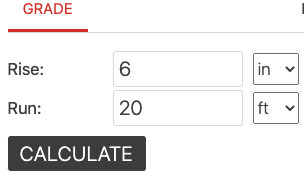
\includegraphics[width=7cm]{../graphics/06Calculator.png}\\
Express your result as follows: \\[0.5cm]
Fraction:\\[0.5cm]
Decimal:\\[0.5cm]
Percentage:\\[0.5cm]
Angle:\\[0.5cm]
\begin{flushright}
  \emph{Not to scale}\\
  \begin{tikzpicture}[xscale=0.3, yscale=3]
    \draw [help lines, xstep=5, ystep=0.5] (0,0) grid (26,1.5);
    \draw [thick, ->] (0,0) -- (28,0) node [below right] {$x$};
    \foreach \x in {5,10,15,20,25}
      \draw[shift={(\x,0)},color=black] (0pt,0pt) -- (0pt,0pt) node[below] {\footnotesize \; $\x$};
    \draw [thick, ->] (0,0)--(0,1.8) node [left] {$y$};
    \foreach \y in {0.5, 1,1.5}
      \draw[shift={(0,\y)},color=black] (0pt,0pt) -- (0pt,0pt) node[left] {\footnotesize \; $\y$};
    \node at (20,0.5) {$\bullet$};
    %\draw [fill] (3,4) circle [radius=0.05] node[above right] {$B(3,4)$};
    \draw [->, thick] (0,0)--(24,0.6);
  \end{tikzpicture}
  \end{flushright}
\end{multicols}
 
\item Find the slope of the line $\overleftrightarrow{AB}$, $A(12,1)$, $B(44,5)$. Use the formula and show the substitution step. Express your result as a fraction, a decimal, and a percent grade.
\begin{multicols}{2}
  $\displaystyle m = \frac{y_B - y_A}{x_B - x_A}$
    \vspace{2cm}
    \begin{flushright}
      \begin{tikzpicture}[xscale=0.1, yscale=1]
        \draw [help lines, xstep=10, ystep=1] (0,0) grid (60,5);
        \draw [thick, ->] (0,0) -- (65,0) node [below right] {$x$};
        \foreach \x in {10,20,...,60}
          \draw[shift={(\x,0)},color=black] (0pt,0pt) -- (0pt,0pt) node[below] {\footnotesize \; $\x$};
        \draw [thick, ->] (0,0)--(0,5.5) node [left] {$y$};
        \foreach \y in {0,1,...,5}
          \draw[shift={(0,\y)},color=black] (0pt,0pt) -- (0pt,0pt) node[left] {\footnotesize \; $\y$};
        \node at (12,1) {$\bullet$};
        \node at (44,5) {$\bullet$};
        %\draw [fill] (3,4) circle [radius=0.05] node[above right] {$B(3,4)$};
        \draw [<->, thick] (6,0.25)--(48,5.5);
      \end{tikzpicture}\\
      \emph{Not to scale}
      \end{flushright}
    \end{multicols}
 
\item Find the equation of the line through the points $(0,2.4)$, $(70,3.8)$. Use the slope formula, then substitute the slope and $y$-intercept into a linear equation.
\begin{multicols}{2}
  $\displaystyle m = \frac{y_2 - y_1}{x_2 - x_1}$, \hspace{1cm} $y=mx+b$
  \columnbreak
  \begin{flushright}
    \emph{Not to scale}\\
    \begin{tikzpicture}[xscale=0.1, yscale=1]
      \draw [help lines, xstep=10, ystep=1] (0,0) grid (70,5);
      \draw [thick, ->] (0,0) -- (75,0) node [below right] {$x$};
      \foreach \x in {10,20,...,70}
        \draw[shift={(\x,0)},color=black] (0pt,0pt) -- (0pt,0pt) node[below] {\footnotesize \; $\x$};
      \draw [thick, ->] (0,0)--(0,5.5) node [left] {$y$};
      \foreach \y in {0,1,...,5}
        \draw[shift={(0,\y)},color=black] (0pt,0pt) -- (0pt,0pt) node[left] {\footnotesize \; $\y$};
      \node at (0,2.4) {$\bullet$};
      \node at (70,3.8) {$\bullet$};
      %\draw [fill] (3,4) circle [radius=0.05] node[above right] {$B(3,4)$};
      \draw [->, thick] (0,2.4)--(75,3.9);
    \end{tikzpicture}
    \end{flushright}
  \end{multicols}

\item Complete each statement about linear equations.
\begin{enumerate}[itemsep=0.5cm]
  \item What is the $y$-intercept of the line $y = 1.25x - 13.5$?
  \item What is the percent grade of the line $\displaystyle y = 0.04x + 12.5$?
  \item What is the slope of a vertical line?
  \item What is the slope of the line $x=7$?

    \item If $m = 4$ then $m_{\perp}=$
    \item Lines $p$ and $q$ have slopes $m_p = -\frac{3}{2}$ then $m_q= +\frac{2}{3}$. Are they parallel, perpendicular, or neither? Justify your answer by showing the product of their slopes.
  \end{enumerate}

\item Is the point $P(55,2.5)$ on the line: $y=0.012x+1.75$? \\[0.5cm]
Support your answer algebraically (substitute $P$'s coordinates into the equation).
\begin{flushright}
  \emph{Not to scale}\\
  \begin{tikzpicture}[xscale=0.1, yscale=1]
    \draw [help lines, xstep=10, ystep=1] (0,0) grid (70,5);
    \draw [thick, ->] (0,0) -- (75,0) node [below right] {$x$};
    \foreach \x in {10,20,...,70}
      \draw[shift={(\x,0)},color=black] (0pt,0pt) -- (0pt,0pt) node[below] {\footnotesize \; $\x$};
    \draw [thick, ->] (0,0)--(0,5.5) node [left] {$y$};
    \foreach \y in {0,1,...,5}
      \draw[shift={(0,\y)},color=black] (0pt,0pt) -- (0pt,0pt) node[left] {\footnotesize \; $\y$};
    \node at (0,1.75) {$\bullet$};
    \node at (55,2.5) {$\bullet$};
    %\draw [fill] (3,4) circle [radius=0.05] node[above right] {$B(3,4)$};
    \draw [->, thick] (0,1.75)--(35,2.17);
  \end{tikzpicture}
  \end{flushright}

\item Quadrilateral $ABCD$ with vertices $A(-2,5)$, $B(0,-1)$, $C(4,0)$, and $D(2,6)$ is shown. \\[0.5cm]
Find the slopes of each side. Is $ABCD$ a parallelogram? a rectangle? Justify your answer.
\begin{multicols}{2}
  Slope of $\overline{AB}=$\\[1.5cm]
  Slope of $\overline{BC}=$\\[1.5cm]
  Slope of $\overline{CD}=$\\[1.5cm]
  Slope of $\overline{AD}=$\\
  \begin{flushright}
    \begin{tikzpicture}[scale=0.8]
      \draw [help lines] (-3,-2) grid (6,7);
      \draw [thick, <->] (-3.4,0) -- (6.4,0) node [below right] {$x$};
      \draw [thick, <->] (0,-2.4)--(0,7.4) node [left] {$y$};
      \draw [thick] (-2,5) node[above left] {$A(-2,5)$}--
        (2,6) node[right] {$D(2,6)$}--
        (4,0) node[below right] {$C(4,0)$}--
        (0,-1) node[below right] {$B(0,-1)$}--
        cycle;
    \end{tikzpicture}
    \end{flushright}
  \end{multicols}

\item Plot a parallelogram (not a rectangle) using Geogebra (use the grid). The legs must not be horizontal or vertical. Paste an image of your work in this Classkick slide from the clipboard or by using the ``camera'' tool.\\[0.25cm]
Spicy: Show the measures the slopes of the quadrilateral sides.

\item 
  \begin{enumerate}
    \item Draw two sides $\overline{AD}$, $\overline{CD}$ to complete a parallelogram $ABCD$. \vspace{0.25cm}
    \item Write the slope of line $\overleftrightarrow{CD}$.
    \begin{multicols}{2}
      
    \item Write the equation of line $\overleftrightarrow{BC}$.\vspace{2cm}
    \item Is $\overleftrightarrow{CD} \perp \overleftrightarrow{BC}$? Show the product of their slopes is or is not $-1$.
    \begin{flushright}
      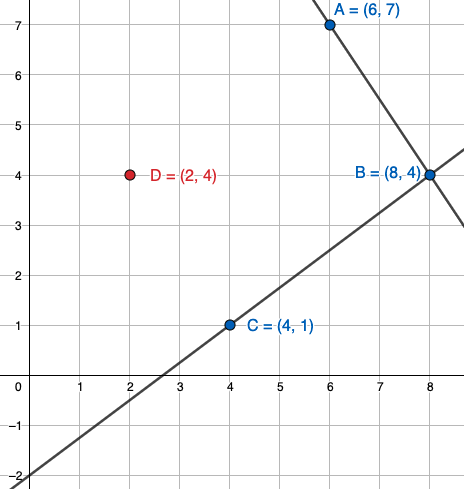
\includegraphics[width=9cm]{../graphics/06Slope-8.png}
    \end{flushright}
    Link: 
    https://www.geogebra.org/calculator/j8kx5ykf
\end{multicols}
\end{enumerate}

\item Find the length of $\overline{DE}$, where $D(1,-5)$ and $E(13,0)$.
       \vspace{4cm}

   \item Determine relationship of each equation to the line  $y=\frac{2}{3} x-6$, circling either parallel, perpendicular, or neither.
     \begin{enumerate}
       \item $2x-3y=6$ \hspace{1cm} Parallel \qquad Perpendicular \qquad Neither
       \vspace{1.5cm}
       \item $3x-2y=5$ \hspace{1cm} Parallel \qquad Perpendicular \qquad Neither
       \vspace{2.cm}
     \end{enumerate}

  \item In the diagram below, $\overleftrightarrow{AC}$ has endpoints with coordinates $A(-1,2)$ and $C(8, -4)$.
    \begin{center} %4 quadrant regents grid
      \begin{tikzpicture}[scale=.48]
        \draw [help lines] (-7,-5) grid (9,7);
        \draw [thick, <->] (-7.4,0) -- (9.4,0) node [below right] {$x$};
        \draw [thick, <->] (0,-5.4)--(0,7.4) node [left] {$y$};
        \draw [thick] (-1,2)--(8, -4);
        \draw [fill] (-1,2) circle [radius=0.1] node[above left] {$A$};
        \draw [fill] (8, -4) circle [radius=0.1] node[below right] {$C$};
      \end{tikzpicture}
    \end{center}
    If $B$ is a point on $\overline{AC}$ and $AB {:} BC = 1{:}2$,  what  are  the  coordinates of $B$?

\newpage
\item $A(2,10)$ is one endpoint of $\overline{AB}$. The segment's midpoint is $M(5,7)$. Find the other endpoint, $B$. \vspace{4cm}

\item In the diagram below, $\triangle ABC$ has vertices with coordinates $A(1,3)$, $B(8,4)$ and $C(4, 7)$.
  \begin{center} %4 quadrant regents grid
    \begin{tikzpicture}[scale=.48]
      \draw [help lines] (-4,-4) grid (9,8);
      \draw [thick, <->] (-4.4,0) -- (9.4,0) node [below right] {$x$};
      \draw [thick, <->] (0,-4.4)--(0,8.4) node [left] {$y$};
      \draw [thick]
        (1,3)node[below]{$A$}--
        (8,4) node[right]{$B$}--
        (4,7) node[above right]{$C$}--cycle;
      %\draw [fill] (-1,2) circle [radius=0.1] node[above left] {$A$};
      %draw [fill] (8, -4) circle [radius=0.1] node[below right] {$C$};
    \end{tikzpicture}
  \end{center}
  Find the length of each side of $\triangle ABC$, showing that it is isosceles and not equilateral.\\[0.5cm]
  \begin{tabular}{c|c|c}
    $AC=$ & $BC=$ & $AB=$ \\
    $\sqrt{(x_C-x_A)^2+(y_C-y_A)^2}$ & $\sqrt{(x_C-x_B)^2+(y_C-y_B)^2}$ & $ \sqrt{(x_B-x_A)^2+(y_B-y_A)^2}$ \\
    & & \\
    & & \\
  \end{tabular}

\end{enumerate}
\end{document}
